% Chapter 4: Diagrama SQL
	\chapter{Diagrama de la base de datos}\label{Chap: Diagrama de la base de datos}
	A continuación se presenta el diagrama de la base de datos generado en SQL Server Managment Studio.
		\begin{figure}[h!]
			\centering
			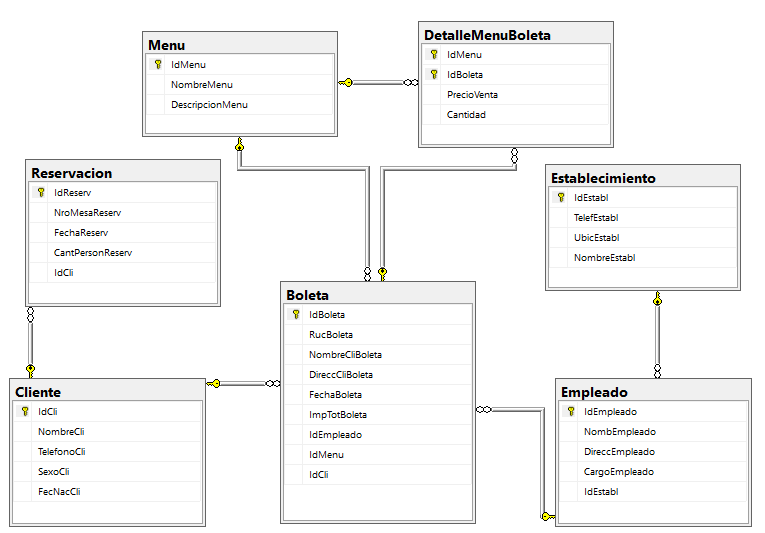
\includegraphics[scale = 0.8]{DiagramSQL2.png}
			\caption{Diagrama de la base de datos}
			\label{fig: Diagrama de la base de datos}
		\end{figure}
	
	La lectura del diagrama de la base de datos es lo siguiente: un cliente puede realizar muchas reservaciones y una reservación puede ser realizado solamente por un cliente; un cliente puede tener muchas boletas y una boleta le pertenece solamente a un cliente; una boleta puede ser emitido por un empleado y un empleado puede emitir muchas boletas; un empleado labora solamente en un establecimiento y en un establecimiento laboran muchos empleados; una boleta puede registrar muchos menús y un menú se puede registrar en muchas boletas.	
		
	